%%%%%%%%%%%%%%%%%%%%%%%%%%%%%%%%%%%%%%
% yale_thesis.tex
% Elena Gramellini
% Started: 2017/12/05
%
% A bare, sample template for a Yale PhD thesis using yalephd.cls
%%%%%%%%%%%%%%%%%%%%%%%%%%%%%%%%%%%%%%

\documentclass[letterpaper,12pt]{yalephd}
% remove draft option for final printing.
% font size must be between 10pt-12pt.

\usepackage{geometry} % you need this for yalephd.cls to work.
\usepackage{graphicx} % you probably want the rest of these.
\usepackage{dcolumn}
\usepackage{bm}

\usepackage{mathtools}
\DeclarePairedDelimiter\bra{\langle}{\rvert}
\DeclarePairedDelimiter\ket{\lvert}{\rangle}
\DeclarePairedDelimiterX\braket[2]{\langle}{\rangle}{#1 \delimsize\vert #2}

\usepackage{multirow}
\usepackage{amsmath}
\usepackage{amsfonts}
\usepackage{amssymb}
\usepackage{appendix}
\usepackage{comment}
\usepackage{cite}
\usepackage{color}
\bibliographystyle{plain}
\usepackage{slashed}  

\newenvironment{dedication}
  {%\clearpage           % we want a new page          %% I commented this
   \thispagestyle{empty}% no header and footer
   \vspace*{\stretch{1}}% some space at the top
   \itshape             % the text is in italics
   \raggedleft          % flush to the right margin
  }
  {\par % end the paragraph
   \vspace{\stretch{3}} % space at bottom is three times that at the top
   \clearpage           % finish off the page
  }




\begin{document}

% Need to define title before the abstract.
\title{Measurement of the positive kaon-argon total hadronic differential cross section in the LArIAT experiment}
\author{Elena Gramellini}
\advisor{Bonnie T. Fleming}
\date{Date you'll receive your degree} % usually not \today.

% All the stuff at the front of your thesis.
\frontmatter

\begin{abstract}
Abstract goes here. Limit 750 words.
\end{abstract}


\maketitle
\makecopyright{2017}

%  \begin{dedication}
%A mia mamma e mio babbo,\\
%grazie per le radici e grazie per le ali.
%    \par   %% or a blank line
%    \vspace{2\baselineskip}
%To my mom and dad,\\
%thank you for the roots and thank you for the wings.
%    \vspace{\baselineskip}
%  \end{dedication}
\tableofcontents
\listoffigures % remove this if you have no figures.
\listoftables % remove this if you have no tables.

\chapter{Acknowledgements} % this needs to be before \mainmatter.
A lot of people are awesome. But not you, who are reading my thesis before it's done.
%The truth is, younger Elena was a theorists at heart and didn't know. She absolutely loved QFT. But, she hated every single person of her class who self-identified as a theorist. She swore never to become one of them and buried that love deep in her heart, never to be touched by those jerks who traded in Lagrangians and measurements of each other's dicks. Was that love not strong enough to overcome the filth of the everyday shade?  Was she not armored enough to shield from other people?s low self-esteem? Who?s fault was that? Not the theorist?s? she always thought it was hers, but was it?  I don?t know. But sure, younger Elena had to find a way to get by. And she did. Painfully, with a lot of bruises and an ocean across. But she did.

% Starts proper arabic numbering of pages and chapters.
\mainmatter

`\chapter{Introduction}\label{ch:-1}

This thesis work concerns the first measurement of the  ($\pi^-$-Ar)  total hadronic cross section  in the 100-1000 MeV  kinetic energy range and the first measurement of the ($K^+$-Ar) total hadronic cross section  in the 100-650 MeV  kinetic energy range. We performed these measurements at the LArIAT experiment,  a small (0.25 ton)  Liquid Argon Time Projection Chamber (LArTPC) on a beam of charged particles at the Fermilab Test Beam Facility.  Albeit particle and nuclear physics have a long history of hadronic cross section measurements, the work outlined in this thesis presents a new methodology -- the ``thin slice method" -- for cross section measurements in argon, possible only thanks to the detection capabilities of the LArTPC technology. The combination of fine-grained tracking and excellent calorimetric information provided by the LArTPC technology  allows to see unprecedented details of particle interactions in argon and, in LArIAT, to measure the kinetic energy of a hadron at each step of the tracking. A renewed interest for precision measurements of hadronic cross sections, particularly in argon, arises from the current  panorama of experimental  particle physics at the intensity frontier.

The discovery of the Higgs boson in 2012 marked the triumph of the Standard Model of Particle Physics; exploring what lays beyond is the real challenge in our field today. 
Since their formulation in 1930, neutrinos have been a source of surprises (and Nobel Prizes) for particle physicists, tiny cracks in our understanding of Nature. In particular, the discovery of neutrino oscillation represents the first evidence of physics Beyond the Standard Model (BSM).  From a theoretical point of view, the field is developing new theories to account for the small but non-zero mass of neutrinos, while trying to remain consistent with the rest of the Standard Model.  From an experimental point of view, we are developing technologies and huge collaborations to probe these theories. As we enter the era of precision measurements of neutrino interaction, neutrinos might hold the key to the next generation of discoveries in particle physics.

Experimentally, precision measurements can be achieved only if the detector technology is able to resolve the fine details of a statistically relevant number of interactions. 
With ``fine details" here we mean the ability to distinguish the many products of the neutrino interaction, such as protons, pions, muons and electrons, and to measure their energy.
Historically,  bubble chamber neutrino detectors were the first revolution in neutrino detection: for example, the spatial resolution of Gargamelle allowed the discovery of neutrino neutral current interaction. Despite the high precision of bubble chambers images, this technology is hard to scale to massive size, making statistical analyses on neutrino interactions almost impossible to perform. To make up for the small neutrino interaction cross section, neutrino experiments moved to very large size, at the expenses of spatial precision. This is the case for the detectors which discovered neutrino oscillation:  both Super-Kamiokande and SNO are massive Cherenkov detectors. With LArTPCs, the field is gaining again bubble-chamber like precision but at massive scales. Following the recommendations of  the latest Particle Physics Project Prioritization Panel  \cite{P5}, the US particle physics panorama is directing a substantial effort towards the exploration of the intensity frontier through the construction of massive LArTPCs. In particular, the near future will see the development of a Short Baseline Neutrino Program (SBN) and long baseline neutrino program  (DUNE), both based on the LArTPC detector technology. The US liquid argon program has the potential to answer many of the fundamental open questions in particle physics today, such as: is there a fourth generation neutrino? is CP violated in the lepton sector? are there any additional symmetries? and, can we find an indication of Grand Unified Theories? 

The SBN program at Fermilab is tasked with conclusively addressing the existence of a fourth neutrino generation in the  $\Delta m^2= \Delta m^2_{14} \sim [0.1 - 10]$ eV$^2$ parameter space. The SBN program entails three surface LArTPCs positioned on the Booster Neutrino Beam at different distances from the neutrino production in oder to fully exploit  the L/E dependence of the oscillation pattern:  SBND (100 m from the decay pipe), MicroBooNE (450 m), and ICARUS (600 m). SBN will also perform an extensive 
program of neutrino cross section measurements, fundamental to abate systematics in the oscillation analyses in both SBN and DUNE.

DUNE has a vast neutrino and non-accelerator physics reach. For what it concerns neutrino physics, oscillation analyses in DUNE have the capability of solving the mass hierarchy and octant problem,  and discovering CP violation in the neutrino sector. Besides its neutrino program, DUNE can open an experimental window on Grand Unified Theories (GUTs). GUTs could potentially answer fundamental questions such as the existence of non-zero neutrino masses and matter-antimatter asymmetry, explaining some ``accidents" in the Standard Models, such as the exact cancellation of the  proton and the electron charge.   Directly probing GUTs at the unification energy scale is impossible by any foreseeable collider experiment. We then need an indirect proof such as baryon number violation, which is predicted by almost every GUT in the form of proton decay, bounded nucleon decay or $n-\bar n$ oscillations on long time-scales. Historically, the main technology used in these searches has been water Cherenkov detectors, with Super-Kamiokande setting all the current experimental limits on the decay lifetimes at the order of $\sim 10 ^{34}$ years. The DUNE far detector and its non-accelerator physics program is a interesting new actor on this stage.  LArTPCs can in fact complement nucleon decay searches in modes where water Cherenkov detectors are less sensitive, especially $p\rightarrow K^+\bar{\nu}$  \cite{Adams:2013qkq}.


Such a diverse physics program speaks to the versatility of the LArTPC technology. LArTPCs provide excellent electron/photon separation \cite{Acciarri:2016sli} lacking in Cherenkov detectors which can be leveraged to abate the photon background from neutral current interactions  in $\nu_e$ searches. LArTPCs also share superb tracking capability with bubble chamber detectors, with several additional benefits. They are electronically read out and self triggered detectors; they provide full 3D-imaging with millimeter resolution, precise calorimetric reconstruction and excellent particle identification. %Plus, female physicists are actually writing code and running experiments, not (only) staring at images \textcolor{red}{-- Too much? --} \cite{2006physics4152G}. 

The amount of information a LArTPC can provide makes these detectors rather complex: a series of dedicated measurements is necessary to obtain meaningful physics results from a LArTPC. The complexity of the LArTPC technology for neutrino detection is due to several reasons. Argon is a fairly heavy element, which means that nuclear effects play an important role in the looks of the interaction topology. For example, pions are one of the main products of neutrino interactions; yet,  since data on charged particle interaction in argon is scarce, neutrino event generators have big uncertainties in the re-scattering simulation of hadrons in argon. %No measurement of hadronic cross sections for pions or kaons is available for argon (yet). 
The amount of details in an LArTPC event is easily  parsed by human eye, but can make automatic event reconstruction rather challenging. Thus, reconstruction algorithms in LArTPC need to be tune to recognize the different topologies of the neutrino interaction products in argon. This is particularly true for pions, since they are an abundant product of the neutrino interactionsl the occurrence of a pion interaction in argon can modify the topology of the neutrino event, causing a misidentification of the neutrino interaction.

The LArIAT \cite{Cavanna:2014iqa} experiment is performing precise cross section measurements of charged particles in argon to bridge this gap of knowledge. 
The LArIAT LArTPC sits on a beam of charged particles at the Fermilab Test Beam Facility; the beam provides charge particles of the type and energy range relevant for neutrino interaction of both SBN and DUNE. The ($\pi^-$-Ar) hadronic cross section is a fundamental input for neutrino detectors in liquid argon, as pion interactions can modify the topology and energy reconstruction of neutrino events in the GeV range, where pion production is abundant. The  ($K^+$-Ar) total hadronic differential cross section in LArIAT is particularly relevant for a high identification efficiency in the context of proton decay searches in DUNE in the  $p\rightarrow K^+\bar{\nu}$  channel. In fact, the kaon-argon cross section affects the kaon topology by modifying the kaon tracking and energy reconstruction, impacting the basis for kaon identification in a LArTPC.  
The cross section analyses exploit the totality of LArIAT's experimental handles; they rely on beam line detector information as well as both calorimetry and tracking in the TPC. These analyses are LArIAT's first physics results. 
In order to measure total hadronic  argon cross sections, several steps are necessary. The analysis starts by identifying a sample of the hadron of interest in the beam line and assessing the beam line contaminations. It proceeds with tracking the hadron candidates in the TPC and measuring their calorimetry at each point in the tracking: the fine sampling of an hadron in the TPC forms the set of ``incident" hadrons.  Then, the hadronic interaction point is identified and the raw cross section is calculated. Two correction\\

This body of work is divided in 8 chapters.
We provide a description of the theoretical framework for the measurements in  Chapter \ref{ch:TheTheory}. Chapter \ref{ch:2} outlines the LArTPC detector technology, while
Chapter \ref{sec:experimentDescription} describes LArIAT experimental setup. We present the event selection for both the pion and kaon analyses, as well as the ``thin-slice method" in Chapter \ref{ch:Interactions}.  Chapter \ref{ch:samples}  describes the work done on the data and Monte Carlo samples in preparation of the cross section analyses.
Chapter \ref{ch:PionXS} shows  the results for the ($\pi^-$-Ar) total hadronic cross section measurement. Chapter \ref{ch:KaonXS} shows  the results for the ($K^+$-Ar) total hadronic cross section measurement. We draw the final remarks on this work in Chapter \ref{ch:Conclusions}

A series of additional studies and calibrations were necessary to perform the cross section analyses. Appendix \ref{ch:AppendixB} shows a measurement of the LArIAT LArTPC electric field using cosmic data. Appendix \ref{ch:AppendixB} shows an optimization of the tracking algorithms geared towards maximizing the efficiency of finding the hadronic interaction point. Appendix \ref{ch:AppendixB} shows the calorimetry calibration of the LArIAT LArTPC, which is a pivotal measurement to enable any physics analysis with TPC data.  



\chapter{Liquid Argon Detectors at the Intensity Frontier}\label{ch:1}


In the next few years, LArTPC experiments -- such as the Short-Baseline Neutrino program (SBN) and DUNE -- will be major players in the intensity frontier field. 

\section{The SBN Program}
\subsection{SBN Goals}
\subsection{Neutrino Interactions and Detection }

\section{DUNE}
\subsection{DUNE Non-Accelerator Physics Program}
\subsection{Rare Decay Searches: Experimental Limit}
\subsection{Nucleon Decay Detection in LAr}

\section{Liquid Argon Time Projection Chambers at the Intensity Frontier}

%Bubble-chamber experiments played a key role in probing the properties of ?-interactions. The Liquid Argon Time Projection Chambers (LArTPC) technology,  first proposed by C.Rubbia in 1977 with ICARUS project [14], is considered the modern evolution of bubble-camber concept, with the additional features of three-dimensional event reconstruction, high-resolution calorimetry, active mass coincident with detector sensitive mass and can intrinsically supply a trigger signal (self-triggering) by means of the scintillation light produced in the liquid noble gas. This technology is ideal to perform $\nu$-studies in a broad energy range, from MeV up to few GeV, with high event reconstruction efficiency, thanks to the capability of particle identifcation and detailed reconstruction of different interaction topologies. In Figure 1.4 is shown a neutrino interaction event, producing a proton, a pion and a muon, as seen in a bubble chamber and in a LArTPC.


\subsection{Time Projection Chamber}
\subsection{Ionization Detectors with Noble Liquids}
\subsection{LArTPC: Principles of Operation}
\subsection{Liquid Argon Ionization Charge Detection}
\subsubsection{Electron Life Time \& purity}
\subsubsection{Space Charge Effect}
\subsubsection{Recombination Effect}
\subsection{Liquid Argon scintillation Light Detection}
\subsubsection{LAr Scintillation Process}
\subsubsection{Wavelength Shifting of LAr Scintillation Light}
\chapter{LArIAT: Liquid Argon In A Testbeam}
\section{LArIAT \& the Intensity Frontier}
\section{Testbeam and Beamline Detectors}
\section{In the Cryostat}

\subsection{TPC: Charge Collection}
\subsection{TPC: Light Collection System}
\subsection{Cryogenics and Purity Control}
\subsection{TPC: Electric Field Measurement}
\section{Trigger and DAQ}
\section{Control Systems}

\chapter{Kaon Interactions in Argon}
Your first chapter is probably an introduction. But who knows.
\chapter{Data Collection}
Your first chapter is probably an introduction. But who knows.
\chapter{LArIAT Monte Carlo}
\section{Beamline}
\subsection{G4Beamline}
\subsection{Data Driven MC}
\label{sec:DDMC}
\section{TPC MC}

\chapter{Energy Calibration}
Your first chapter is probably an introduction. But who knows.
\chapter{Tracking Optimization}
Understanding how kaons and pions are tracked inside the TPC and optimizing the reconstruction algorithms to maximize the correct identification of the interaction point is a fundamental step of the analysis. 


\section{MC sample and WC2TPC match}
The optimization is performed on a MC sample of 191000 kaons and 359000 pions produced with the DDMC technique. DDMC particles are shot from the WC4 location into the TPC following the beam profile.
We mimic the matching between the WC and the TPC track on Monte Carlo by constructing a fake WC track using truth information at wire chamber four. We then apply the same WC to TPC matching algorithm as in data. 

Plots I want in this section:
\begin{enumerate}
\item WC2TPC MC DeltaX, DeltaY and $\alpha$
\item Delta L, reco - true
\item Delta L, reco - true Elastic, Delta L, reco - true Inelastic, other
\item Length Quality cut
\item Efficiency as a function of true KE and Angle
\end{enumerate}





\section{Wire chamber-to-TPC match}
\subsection{Wire chamber-to-TPC match: importance and definition}
\textcolor{red}{something something about why this match is important}

%In data, we attempt to uniquely match one WC-Track to one and only one reconstructed TPC track. This match is done by using in the $X$ and $Y$ coordinate of the extrapolated WC-Track to the upstream most point of the reconstructed TPC Track and by using the angle between the incoming track angle and the reconstructed TPC. We define $\Delta$X as the difference between the $x$ position of the most upstream point of the TPC track and the $x$ position of the WC track as projected to the TPC front face. $\Delta$Y is defined analogously. We define  $\Delta$R as $ \Delta \text{R} =  \sqrt{ \Delta \text{X}^2 +  \Delta \text{Y}^2}  $. The angle between the incident WC Track and the TPC track in the plane that contains them defines $\alpha$.  

%We define a match between WC-track and TPC reconstructed track if  $\Delta \text{R} < r_{T}$, $\alpha < \alpha_{T}$ and the Z position of the first reconstructed point of the TPC track is within 2 cm from the TPC front face. The determination of the best $r_{T}$ and $\alpha_{T}$ is the scope of the following section.

%In MC, we mimic the matching between the WC and the TPC track on Monte Carlo by constructing a fake WC track using truth information at wire chamber four. We then apply the same WC to TPC matching algorithm as in data. 

\subsection{Matching optimization}\label{ch:WC2TPCMatchOptimization}
Scope of this optimization study is assessing the goodness of the wire chamber-to-TPC match on Monte Carlo and porting the optimized selection cuts to data. A word of caution is necessary here. With this study, we want to minimize pathologies associated with the presence of the primary kaon itself, like the incorrect association between the beamline kaon its decay products inside the TPC.  Assessing the contamination from pile-up\footnote{We remind the reader that the DDMC is a single particle Monte Carlo, where the beam pile up is not simulated.}, albeit related, is beyond the scope of this study.

In MC, we are able to define a correct WC2TPC match using the Geant4 truth information. We are thus able to count how many times the WC tracks is associated with the wrong TPC reconstructed track. 

%We define two populations: TPC tracks correctly matched and one of all the other match.
We define a correct match if the all following conditions are met:
\begin{itemize}
\item[-] the length of the true primary Geant4 track in the TPC is greater than 2 cm,  
\item[-] the length of the reconstructed track length is greater than 2 cm,
\item[-] the Z position of the first reconstructed point is within 2 cm from the TPC front face
\item[-] the distance between the reconstructed track and the true entering point is the minimum compared with all the other reconstructed tracks.
\end{itemize}

In order to count the wrong matches, we consider all the reconstructed tracks whose Z position of the first reconstructed point lies within 2 cm from the TPC front face. Events with true length in TPC $<$ 2 cm are included. 
Since kaons are shot 100 cm upstream from the TPC front face, the following two scenarios are possible from a truth standpoint: 
\begin{itemize}
\item[[$Ta$]] the primary kaon decays or interact strongly before getting to the TPC,
\item[[$Tb$]] the primary kaon enters the TPC.
\end{itemize}

Once we choose the selection cuts to determine a reconstructed wire chamber-to-TPC match $r_{T}$ and $\alpha_{T}$, the following four scenarios are possible : 
\begin{itemize}
\item[1)] no reconstructed tracks are matched
\item[2)] the correct track and one (or more) wrong tracks are matched
\item[3)] only the correct track is matched
\item[4)] one (or more) wrong track is matched.
\end{itemize}

If we keep only events with one and only one match, we discard cases 1) and 2) from the cross section measurement. For each set of $r_{T}$ and $\alpha_{T}$ selection value, we define purity and efficiency of the selection as follows:
\begin{equation}
\text{Efficiency} = \frac{\text{Number of events correctly matched}}{\text{ Number of events with primary in TPC}}
\end{equation}

\begin{equation}
\text{Purity} = \frac{\text{Number of events correctly matched}}{\text{Total number of matched events}}.
\end{equation}

Figure \ref{fig:EffPurityK} shows the efficiency (left) and purity (right) for wire chamber-to-TPC match as a function of the radius, $r_{T}$, and angle, $\alpha_{T}$, selection value. It is apparent how both efficiency and purity are fairly flat as a function of the radius selection value at a given angle. This is not surprising, given the fact that the wrong matches can occur  in a single particle gun MC  only for mis-tracking of the primary or for association with decay products, which are generally different in angle, but might be more similar in $x$ and $y$ projection. The radius cut would play a key role in removing pile up events. 

For LArIAT cross section measurements, we generally prefer purity over efficiency, since a sample of particle of a pure species will lead to a better measurement. In the case of kaons however, efficiency needs not to drop too low, given the smallness of the kaon sample. We choose $(\alpha_{T}$, $r_{T}) = (8 \text{ deg}, 4 \text{ cm} )$ and get a MC 85\% efficiency and 98\% purity.


\begin{figure}[hpbt]
\centering
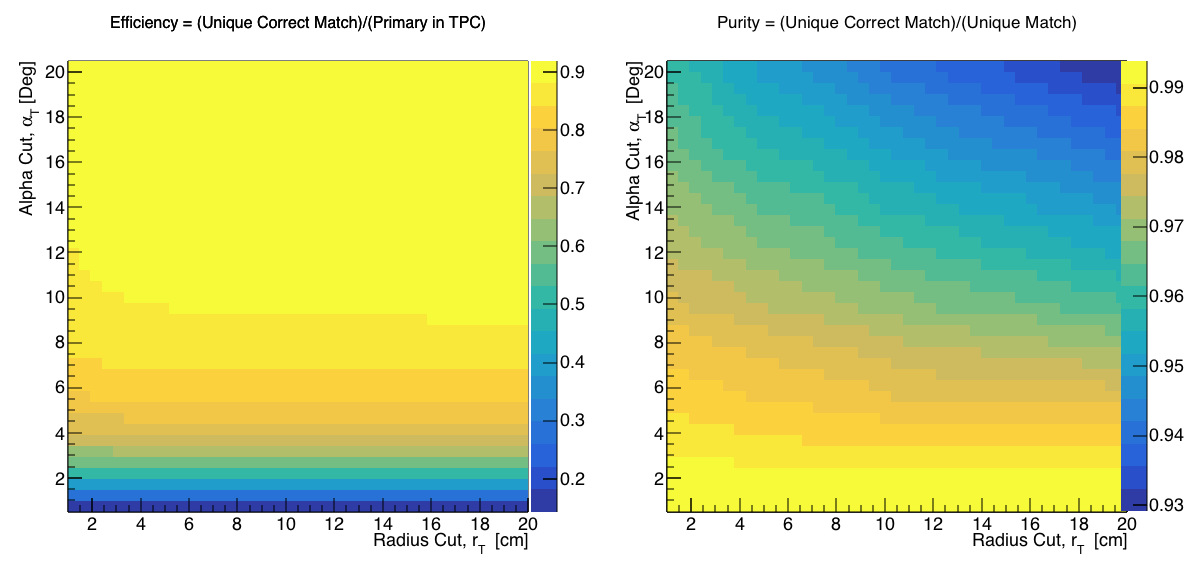
\includegraphics[width=15cm]{Chapter-6/Images/KEffPurity.png}
\caption{Efficiency (left) and purity (right) for wire chamber-to-TPC match as a function of the radius and angle selections.}
\label{fig:EffPurityK}
\end{figure}

\subsection{Porting optimization to data}

\chapter{Kaon Cross Section Measurement}
Your first chapter is probably an introduction. But who knows.


% Add additional \chapter{}s as necessary.

% use \cite{} to cite a reference in your bibliography file.
% use \ref{} to reference a \label{} from an equation, figure, or table.

% for sets of equations use align:
%\begin{align}
%\end{align}

% for figures:
%\begin{figure}[ht]
%\centering
%\includegraphics[width=.45\textwidth]{name_of_figure.eps}
%\caption{A caption! \label{a_figure}}
%\end{figure}

% for tables:
%\begin{table}
%\begin{tabular}{c|c|c}
% 1 & 2 & 3 \\
%\hline
%\end{tabular}
%\caption{Another caption! \label{a_table}}
%\end{table}

% Only call appendix once, here.
\appendix
\chapter{Measurement of LArIAT Electric Field}

\chapter{Construction of A Cosmic Ray Tagger for MicroBooNE}

\chapter{Pion Analysis}

\subsection{Data Sample}

We decided to use only the data from the  -60 A, -100 A RunII configurations, because the beam composition for these 2 beamline configurations is available in G4Beamline. Run II data is better than Run I in terms of calorimetry and understanding of the detector. 

The used SamWeb definition is PionAna\_RunII\_60A\_100A\_lovely1\_elenag\_00  = 

Defined as ``defname: Lovely1 and data\_tier digits and lariat\_mid\_f\_mc7anb < 0 and create\_date < '2017-06-02' and run\_number != 9276 and run\_number != 9277 and run\_number != 8836 and run\_number != 9083 and run\_number != 9122 and run\_number != 8977 and run\_number != 8981 and run\_number != 8982 and run\_number != 8983 and run\_number != 8984 and run\_number != 8985 and run\_number != 8991 and run\_number != 8994 and run\_number != 8996 and run\_number >= 8767 and
run\_number <= 9635"

\begin{table}[]
\centering
\caption{My caption}
\label{my-label}
\begin{tabular}{|c|c|c|c|}
\hline
Stage                                          & -100A +64 GeV & -60A +64 GeV & Number of Evt \\
\hline
SamWebDefinition                     & 32.7\%        & 67.3\% & 3569206      \\
WCQuality                                  & 37.8\%        & 63.2\% &  553486      \\
P$_{WC4} > $ 420 MeV/c               & 50.8\%        & 49.2\% &  423294      \\
TOF Cut                                     & 32.7\%        & 67.3\% &       \\
\hline
                                               &               &             &\\
\hline
\end{tabular}
\end{table}

\subsection{Capture and Decay}
Our goal is to measure the total hadronic cross section for negative pions in argon. Since pion capture can be classified as an electromagnetic process and pion decay is a week process,  capture and decay represent unwanted interactions in our sample. We present here a study of capture and decay in Monte Carlo and the solution we adopted to mitigate their present in our sample. 

For this MC study, we use a sample of 359000 MC pions generated according to the beam profile with the DDMC described in \ref{sec:DDMC}. Unlike decay -- which may occur both in flight and at rest -- capture occurs predominantly
at rest. Thus, we can highly mitigate capture and decay at rest by removing pions whose energy is low enough to stop in the TPC. This translates into a momentum selection, where we keep only events whose WC momentum is above a certain threshold. 
Figure \ref{fig:CaptureMom} shows the true momentum distribution for the primary\footnote{We use here the Geant4 denomination "primary" to indicate that the pion considered does not undergo interactions modifying its energy before getting to the TPC. In fact, not every pion shot from wire chamber four will arrive to the TPC as primary,  some will decay or interact before the TPC, as explained in \textcolor{red}{reference to WC 2 TPC chapter}} pions that arrive to the TPC (pink), that capture (green) or decay (blue) inside the TPC, on a linear and log scale vertical axis. 

\begin{figure}[hpbt]
\centering
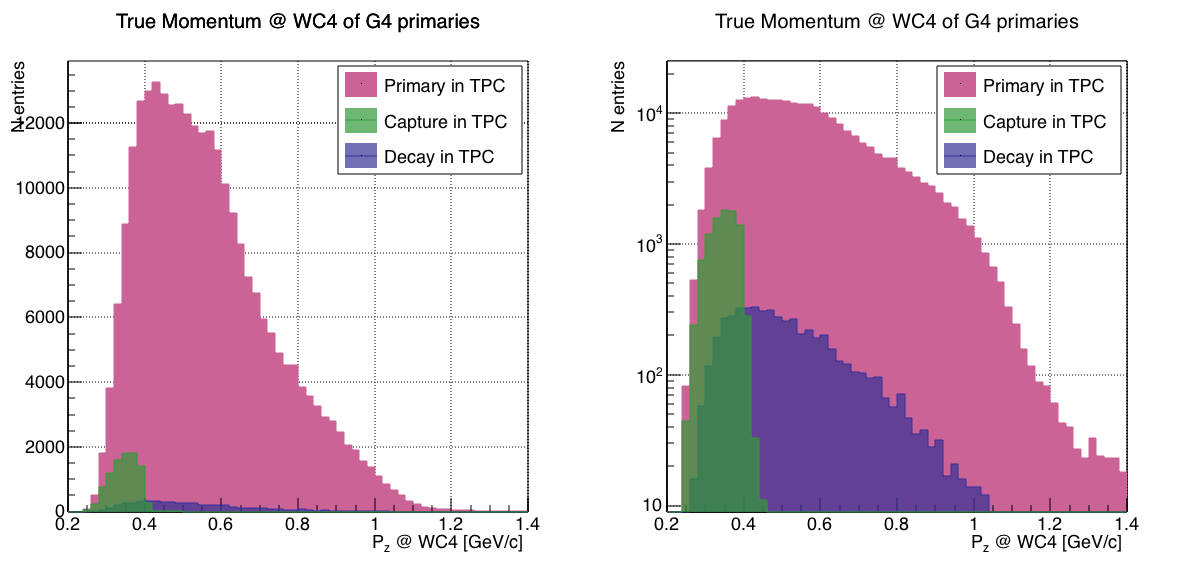
\includegraphics[width=15cm]{Chapters/C-PionImages/CDAsMomentumFunct.png}
\caption{True momentum distribution at wire chamber 4 for every simulated pion arriving in the TPC (pink), ending its life in capture (green) or in decay (blue) in the TPC, linear vertical axis on the left, logarithmic on the right. }
\label{fig:CaptureMom}
\end{figure}


In order to choose the selection value for the wire chamber momentum, it is beneficial to estimate the ratio of events which capture or decay that survive the selection in MC as a function of the momentum threshold, and compare it with the survival ratio for all events. This is done in figure \ref{fig:survRatio}. We define the survival ratio simply  as the number of events surviving the true momentum cut divided by the number of events of that given category. The survival ratio calculated separately for the three event categories explained above: total (pink), capture (green) and decay (blue).
Selecting pions with momentum greater than 420 MeV/c reduces the capture events by ~99\% while maintaining about 80\% of the total data sample. 
Figure \ref{fig:evtRatio} shows the ratio of events which end their life in capture (green) or decay (blue) over the total number of events as a as a function of the true momentum at wire chamber four. This ratio is slightly dependent on the inelastic cross section implemented in Geant4, as we are able to register a pion capture (or decay) only if it doesn't interact inelastically in the TPC. For momenta greater than 420 MeV/c, the percentage of capture events drops below 1\% and the percentage of decays is never above 2\%.

\begin{figure}[h!]
\centering
\begin{minipage}[t]{0.45\textwidth}
\centering
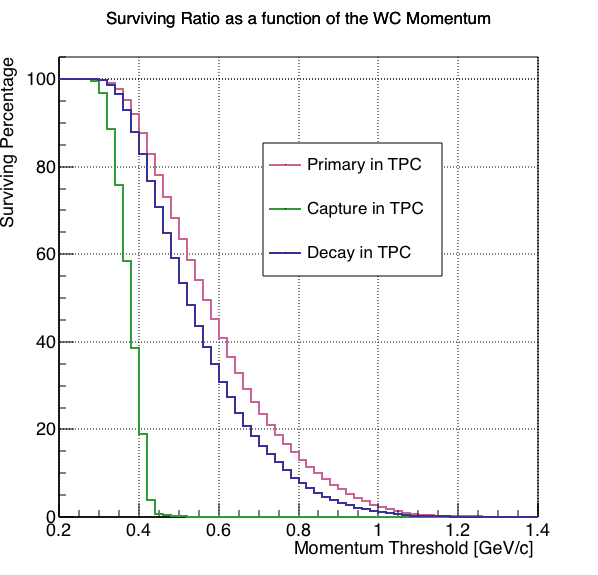
\includegraphics[width=7.5cm]{Chapters/C-PionImages/CDThreshold.png}
\caption{Survival ratio as a function of selection threshold on true momentum at wire chamber four for for every simulated pion arriving in the TPC (pink), capture (green) or in decay (blue).   }
\label{fig:survRatio}
\end{minipage}\hfill
\begin{minipage}[t]{0.45\textwidth}
\centering
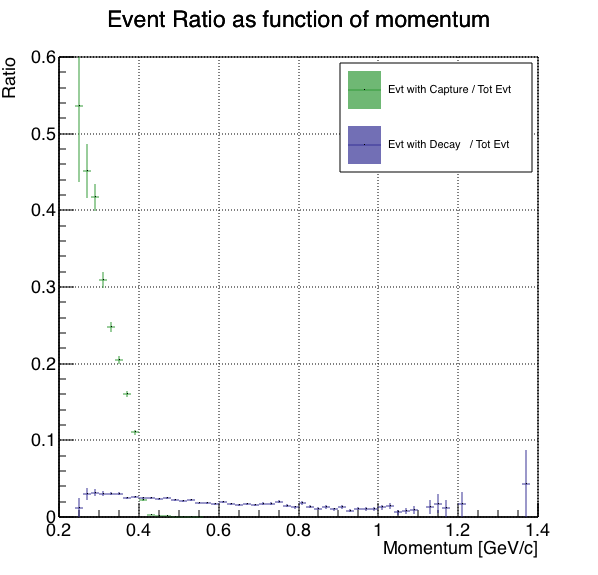
\includegraphics[width=7.5cm]{Chapters/C-PionImages/CDRatio.png}
\caption{Ratio between the capture (green) and decay (blue) events over the total number of events as a as a function of the true momentum at wire chamber four.}
\label{fig:evtRatio}
\end{minipage}
\end{figure}















% Any chapters such as End Notes go after this.
\backmatter

\bibliography{bib.bib}
\bibliographystyle{plain}
% for your own sake, use a bibtex file, so all of the numbering of references will be done
% automatically.

\end{document}
